\documentclass[aspectratio=169]{beamer}
\usetheme{Madrid}
\usecolortheme{default}
\usepackage[utf8]{inputenc}
\usepackage[spanish]{babel}
\usepackage{graphicx}
\usepackage{hyperref}
\usepackage{booktabs}
\usepackage{array}

\usepackage{background}

% Configuración de la marca de agua (logo tenue en esquina inferior derecha)
\backgroundsetup{
	scale=0.45,                % Tamaño más grande para que se note en el centro (prueba 0.35 a 0.55)
	angle=0,                   % Sin rotación (o pon 15 o -15 si quieres un efecto diagonal sutil)
	opacity=0.08,              % Muy tenue (0.06–0.12 para que no moleste el texto)
	contents={
\includegraphics[height=16cm]{cau-logo.png}},  % Aumenta height para mayor visibilidad
	position=current page.center,   % ← ¡CENTRO DE LA PÁGINA!
	% No necesitas vshift ni hshift cuando usas .center
}

% Esto es clave: fuerza que el fondo se aplique en la capa correcta de Beamer
\setbeamertemplate{background}{\BgMaterial}


\title{Normas APA - Séptima Edición}
\subtitle{Citas en el Texto}
\author{Edison Achalma}
\institute{Corporacion Académica Universitaria CAU -UNSCH}
\date{\today}

\begin{document}

\frame{\titlepage}

\begin{frame}{Tabla de Contenido}
\tableofcontents
\end{frame}

\section{¿Qué es una Cita?}

\begin{frame}{Definición de Cita}
\begin{block}{Cita}
Inclusión de ideas, conceptos o información de otras fuentes en nuestro trabajo, con la correspondiente atribución de autoría.
\end{block}

\vspace{0.5cm}
\textbf{Sistema APA:} Autor-Fecha

\end{frame}

\begin{frame}{¿Por qué Citar?}
\begin{itemize}
    \item Dar crédito a los autores originales
    \item Evitar el plagio
    \item Permitir verificación de la información
    \item Mostrar la base teórica del trabajo
    \item Distinguir ideas propias de ideas ajenas
\end{itemize}

\end{frame}

\section{Tipos de Citas}

\begin{frame}{Clasificación de Citas}
% Imagen: Diagrama de árbol mostrando tipos de citas (textual/parafraseo, narrativa/parentética)
\begin{center}
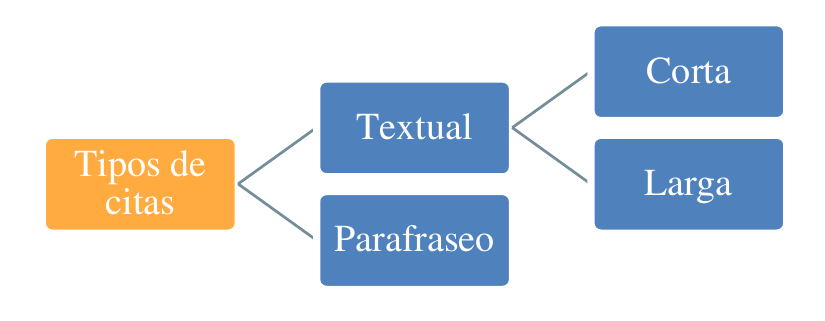
\includegraphics[width=0.85\textwidth]{images/tipos_citas.png}
\end{center}
\end{frame}

\begin{frame}{Cita Narrativa vs Parentética}
\begin{columns}
\column{0.5\textwidth}
\textbf{Cita Narrativa:}
\begin{itemize}
    \item Autor en el texto
    \item Énfasis en el autor
    \item Fecha entre paréntesis
\end{itemize}

\column{0.5\textwidth}
\textbf{Cita Parentética:}
\begin{itemize}
    \item Autor en paréntesis
    \item Énfasis en la idea
    \item Todo entre paréntesis
\end{itemize}
\end{columns}

\end{frame}

\section{Citas Textuales}

\begin{frame}{Cita Textual}
\begin{block}{Definición}
Reproducción exacta de las palabras del autor original
\end{block}

\textbf{Elementos requeridos:}
\begin{itemize}
    \item Apellido del autor
    \item Año de publicación
    \item Número de página (p. o pp.)
\end{itemize}
\end{frame}

\begin{frame}{Cita Textual Corta (menos de 40 palabras)}
% Imagen: Ejemplo completo de cita textual corta narrativa con todos los elementos señalados
\begin{center}
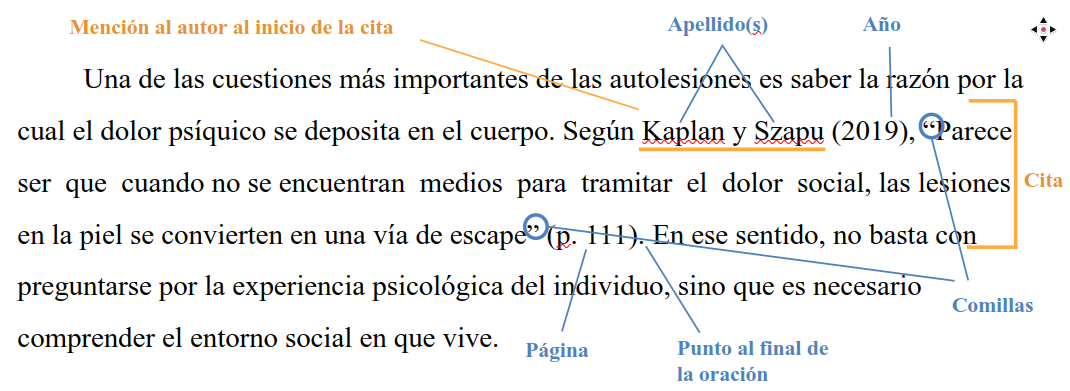
\includegraphics[width=0.85\textwidth]{images/cita_textual_corta_narrativa.png}
\end{center}
\end{frame}

\begin{frame}{Cita Textual Corta Parentética}
% Imagen: Ejemplo completo de cita textual corta parentética
\begin{center}
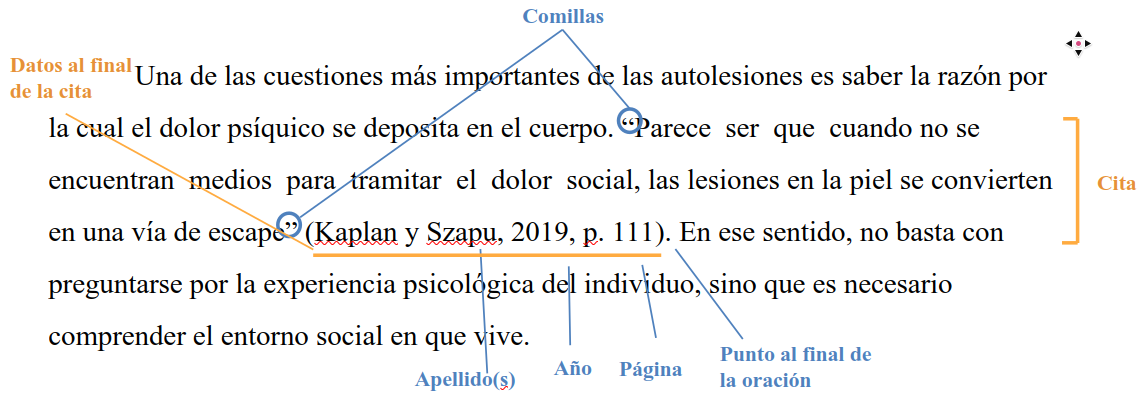
\includegraphics[width=0.85\textwidth]{images/cita_textual_corta_parentetica.png}
\end{center}

\begin{alertblock}{Recordar}
Comillas dobles, punto al final de la oración
\end{alertblock}
\end{frame}

\begin{frame}{Cita Textual Larga (40+ palabras)}
% Imagen: Ejemplo completo de cita textual larga narrativa con sangría
\begin{center}
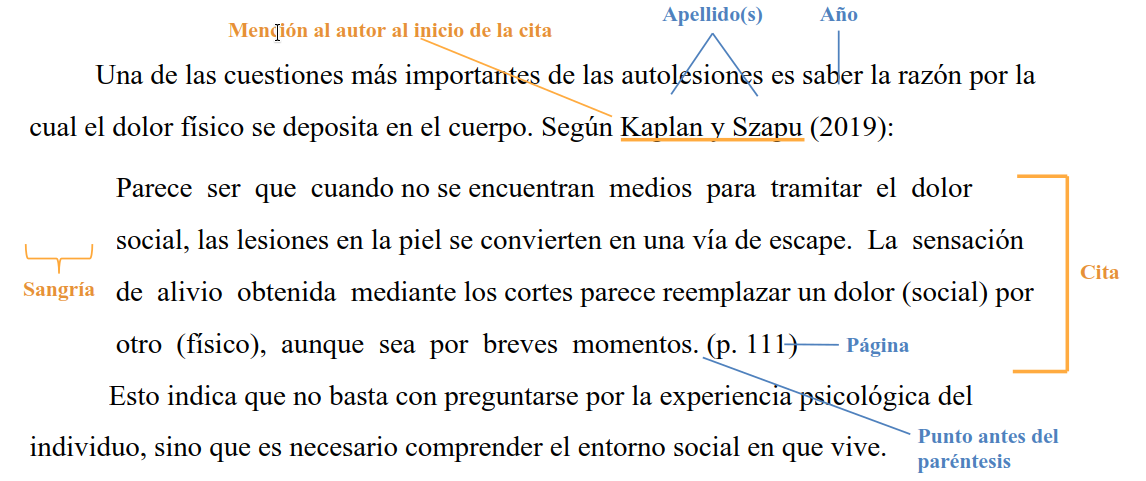
\includegraphics[width=0.8\textwidth]{images/cita_textual_larga_narrativa.png}
\end{center}
\end{frame}

\begin{frame}{Características de la Cita Larga}
\begin{block}{Formato}
\begin{itemize}
    \item Bloque separado del texto
    \item Sangría de 1.27 cm
    \item Sin comillas
    \item Mismo tamaño de fuente
    \item Interlineado doble
    \item Punto ANTES del paréntesis
\end{itemize}
\end{block}
\end{frame}

\begin{frame}{Cita Textual Larga Parentética}
% Imagen: Ejemplo completo de cita textual larga parentética
\begin{center}
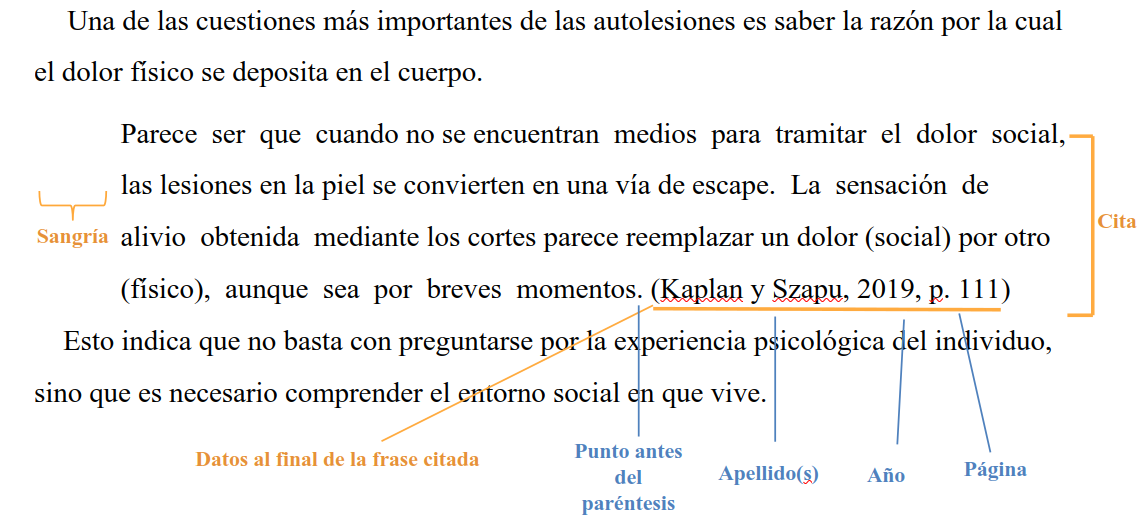
\includegraphics[width=0.8\textwidth]{images/cita_textual_larga_parentetica.png}
\end{center}
\end{frame}

\section{Parafraseo}

\begin{frame}
	\frametitle{¿Qué es el Parafraseo?}
	\begin{definition}
		Exposición o \textbf{explicación} que se realiza sobre un mensaje o las \textbf{ideas del autor citado} utilizando \textbf{nuestras propias palabras}, con el fin de facilitar su comprensión. A esta acción se le conoce como \alert{parafrasear}.
	\end{definition}
	
	\vspace{0.5em}
	
	\begin{itemize}
		\item Es una habilidad crucial en la escritura académica para:
		\begin{itemize}
			\item Evitar el plagio
			\item Clarificar conceptos complejos
			\item Demostrar comprensión profunda del material
		\end{itemize}
	\end{itemize}
	
	\vspace{0.5em}
	
	\begin{alertblock}{Importante}
		Cuando un texto ha sido parafraseado, debe incluirse una cita adecuada indicando la fuente original.
	\end{alertblock}
\end{frame}

\begin{frame}
	\frametitle{Importancia del Parafraseo}
	\begin{columns}[c]
		\begin{column}{0.48\textwidth}
			\begin{block}{¿Por qué parafrasear?}
				\begin{itemize}
					\item Es un proceso \textbf{lingüístico-cognitivo} complejo
					\item Juega un papel central en la apropiación y conservación del conocimiento
					\item Desarrolla el pensamiento crítico
				\end{itemize}
				\vspace{0.3em}
				\small{(Fuchs, 1985)}
			\end{block}
		\end{column}
		
		\begin{column}{0.48\textwidth}
			\begin{block}{¿Para qué parafrasear?}
				\begin{itemize}
					\item Para la construcción del conocimiento
					\item Para demostrar comprensión profunda
					\item Para explicar conceptos complejos de manera accesible
				\end{itemize}
			\end{block}
		\end{column}
	\end{columns}
	
	\vspace{0.5em}
	
	\begin{alertblock}{Competencia clave}
		El estudiante universitario debe ser capaz de \textbf{explicar lo que comprendió con sus propias palabras}.
	\end{alertblock}
\end{frame}

\begin{frame}{¿Qué es Parafrasear?}
\begin{block}{Parafraseo}
Expresar las ideas de otro autor con nuestras propias palabras
\end{block}

\textbf{No es:}
\begin{itemize}
    \item Cambiar algunas palabras por sinónimos
    \item Reordenar las frases
    \item Cambiar la voz (activa/pasiva)
\end{itemize}

\textbf{Sí es:}
\begin{itemize}
    \item Comprender la idea
    \item Reescribirla completamente
    \item Mantener el sentido original
\end{itemize}
\end{frame}

\begin{frame}{Parafraseo Narrativo}
% Imagen: Ejemplo de parafraseo narrativo con texto original y paráfrasis
\begin{center}
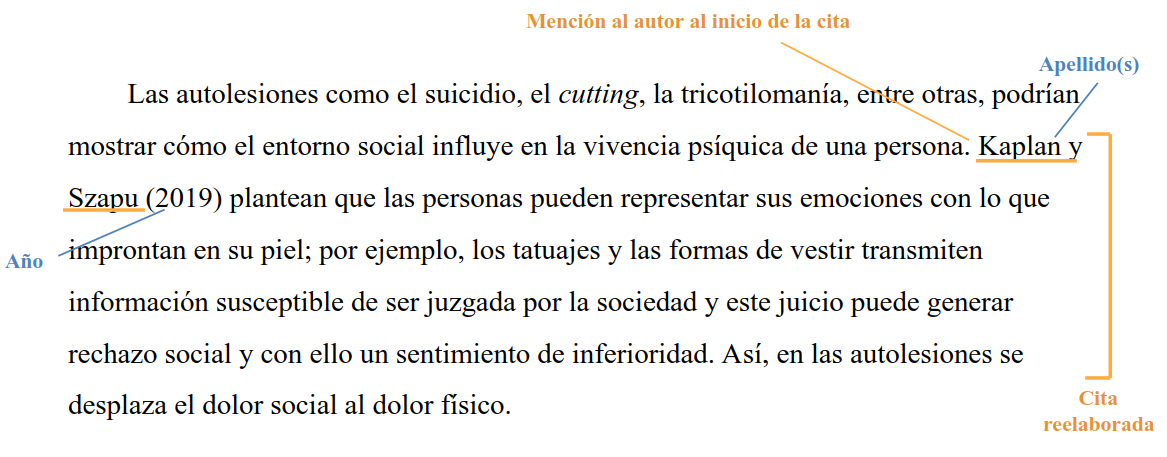
\includegraphics[width=0.85\textwidth]{images/parafraseo_narrativo.png}
\end{center}
\end{frame}

\begin{frame}{Parafraseo Parentético}
% Imagen: Ejemplo de parafraseo parentético
\begin{center}
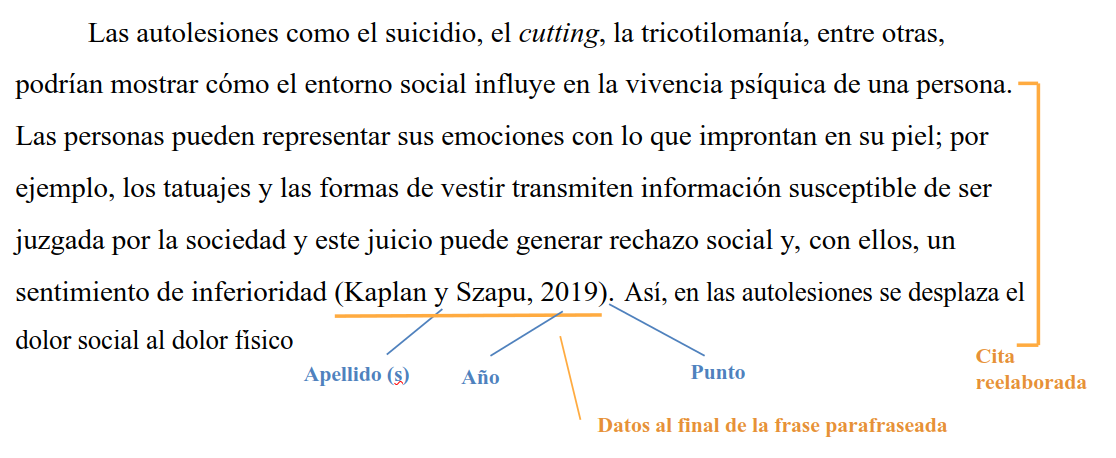
\includegraphics[width=0.85\textwidth]{images/parafraseo_parentetico.png}
\end{center}

\begin{alertblock}{Nota}
En el parafraseo NO es obligatorio incluir el número de página (aunque se puede)
\end{alertblock}
\end{frame}



\begin{frame}
	\frametitle{Tipos de Parafraseo}
	\begin{block}{1. Parafraseo Mecánico}
		\begin{itemize}
			\item \textbf{Sustitución simple} de palabras por sinónimos
			\item Se realizan cambios sintácticos \textcolor{red}{mínimos}
			\item Mantiene estructura similar al texto original
			\item Más sencillo pero menos profundo
		\end{itemize}
	\end{block}
	
	\vspace{0.5em}
	
	\begin{block}{2. Parafraseo Constructivo}
		\begin{itemize}
			\item \textbf{Reelaboración completa} del texto
			\item Se realizan cambios sintácticos \textcolor{blue}{sustanciales}
			\item Conserva el significado pero con estructura diferente
			\item Demuestra mayor comprensión del contenido
		\end{itemize}
	\end{block}
\end{frame}

\begin{frame}
	\frametitle{Proceso de Parafraseo: 6 Pasos}
	\begin{figure}[H]
		\centering
		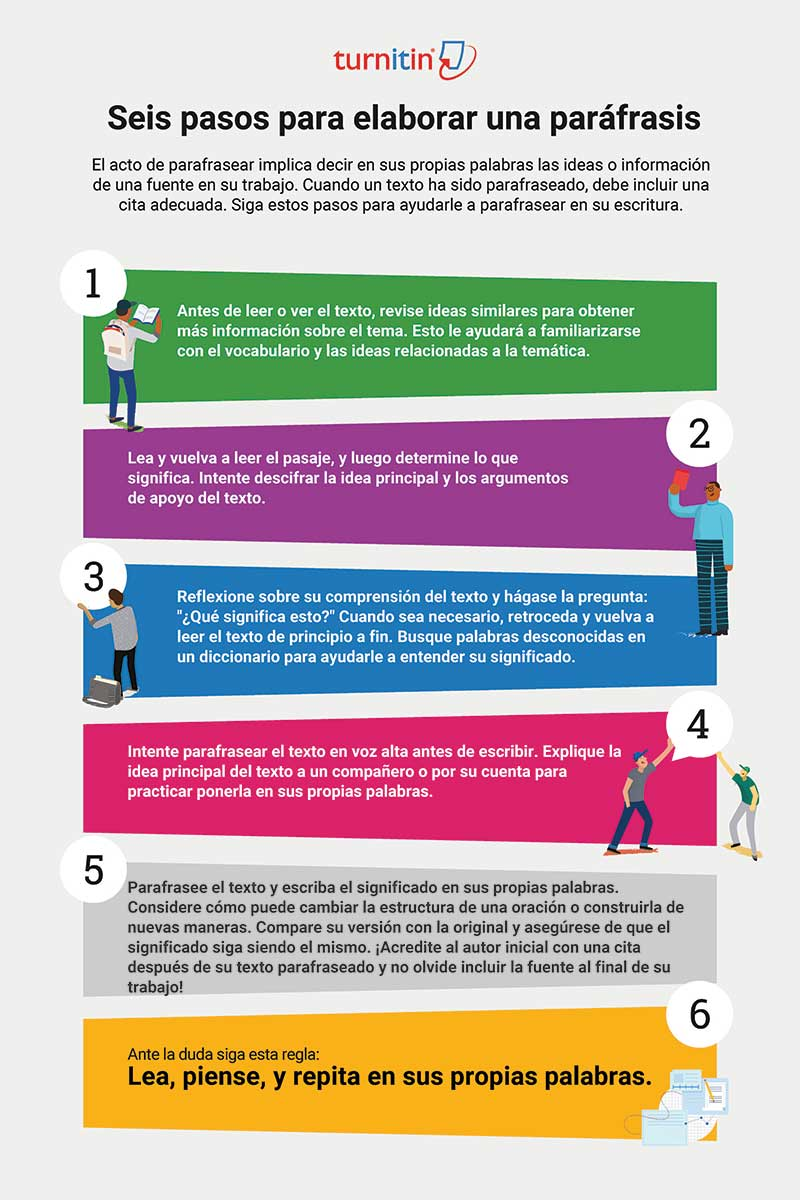
\includegraphics[width=0.5\linewidth]{images/seis-pasos-para-elaborar-una-parafrasis-opt}
	\end{figure}
\end{frame}


\begin{frame}
	\frametitle{Lo que NO se debe parafrasear}
	
	Existen elementos que deben citarse textualmente o presentarse en su forma original:
	
	\begin{itemize}
		\item \textbf{Definiciones técnicas} precisas
		\item \textbf{Leyes científicas} y fórmulas
		\item \textbf{Listas} específicas de elementos
		\item \textbf{Objetivos, hipótesis y conclusiones} de investigaciones
		\item \textbf{Contenido de tablas e infografías}
		\item \textbf{Relaciones causales} complejas
		\item \textbf{Párrafos con alta densidad de términos técnicos} o palabras clave especializadas
	\end{itemize}
	
	\vspace{0.5em}
	
	\begin{alertblock}{Regla general}
		Si parafrasearlo alteraría significativamente el significado o la precisión, es mejor citar textualmente.
	\end{alertblock}
\end{frame}














%\section{Técnicas de Parafraseo}


% EJEMPLOS PRÁCTICOS

\subsection{Ejemplo 1: Liderazgo Situacional}

\begin{frame}[allowframebreaks]
	\frametitle{Ejemplo 1: Identificación de Ideas Clave}
	\framesubtitle{Liderazgo Situacional (Robbins)}
	
	\textbf{PASO 1: Texto Original}
	\begin{block}{}
		\small
		En el análisis de \textbf{Robbins} sobre el comportamiento organizacional, se identifican rasgos del \textbf{liderazgo situacional}, donde el \textbf{líder} adapta su estilo según las circunstancias y el nivel de madurez de sus \textbf{colaboradores}. Este enfoque fomenta que los equipos enfrenten los \textbf{desafíos} con estrategias flexibles, promoviendo una reflexión constante sobre las \textbf{metas organizacionales} y los \textbf{recursos disponibles}. Además, estos líderes no solo responden a las \textbf{necesidades inmediatas}, sino que buscan potenciar el \textbf{desarrollo profesional} de sus seguidores, creando entornos que favorezcan el \textbf{crecimiento sostenible}. (Robbins y Judge, 2013, p.15).
	\end{block}
	
	\framebreak
	
	\textbf{PASO 2: Identificar Ideas Principales}
	\begin{block}{}
		\small
		\textcolor{teal}{En el análisis de \textbf{Robbins} se identifican rasgos del \textbf{liderazgo situacional}}, donde el \textbf{líder} adapta su estilo según las circunstancias y el nivel de madurez de sus \textbf{colaboradores}. \textcolor{olive}{Este enfoque fomenta que los equipos enfrenten los \textbf{desafíos} con estrategias flexibles, promoviendo una reflexión constante sobre las \textbf{metas organizacionales} y los \textbf{recursos disponibles}}. \textcolor{cyan}{Además, estos líderes no solo responden a las \textbf{necesidades inmediatas}, sino que buscan potenciar el \textbf{desarrollo profesional} de sus seguidores}, \textcolor{magenta}{creando entornos que favorezcan el \textbf{crecimiento sostenible}}. (Robbins y Judge, 2013, p.15).
	\end{block}
	
	\framebreak
	
	\textbf{PASO 3: Parafraseo Constructivo}
	\begin{block}{}
		\small
		\textbf{Robbins} destaca en su estudio componentes del \textbf{liderazgo situacional}, en el que el \textbf{líder} ajusta su enfoque según el contexto y las capacidades de sus \textbf{colaboradores}. Esto permite que los equipos aborden los \textbf{desafíos} con soluciones adaptativas, incentivando la evaluación de las \textbf{metas organizacionales} y el uso eficiente de los \textbf{recursos disponibles}. Adicionalmente, estos líderes atienden las \textbf{necesidades inmediatas} mientras impulsan el \textbf{desarrollo profesional}, generando condiciones óptimas para un \textbf{crecimiento sostenible}. (Robbins y Judge, 2013).
	\end{block}
\end{frame}

\subsection{Ejemplo 2: Teoría Económica}

\begin{frame}[allowframebreaks]
	\frametitle{Ejemplo 2: La Mano Invisible}
	\framesubtitle{Teoría Económica de Adam Smith}
	
	\textbf{Texto Original}
	\begin{block}{}
		\small
		El mercado se regula por la mano invisible, un mecanismo que permite que las acciones individuales de los agentes económicos, motivadas por el interés propio, generen beneficios colectivos en forma de equilibrio de oferta y demanda. Este principio sostiene que la libertad de los individuos para perseguir sus objetivos económicos fomenta la competencia, lo que a su vez impulsa la innovación y la eficiencia en la producción. Así, el bienestar social mejora sin necesidad de intervención directa del estado. (Smith, 1776, p.34).
	\end{block}
	
	\framebreak
	
	\textbf{Identificación de Conceptos Clave}
	\begin{block}{}
		\small
		\textcolor{purple}{El mercado se regula por la \textbf{mano invisible}}, un mecanismo que permite que las acciones individuales de los \textbf{agentes económicos}, motivadas por el interés propio, generen beneficios colectivos en forma de \textbf{equilibrio de oferta y demanda}. \textcolor{brown}{Este principio sostiene que la libertad de los individuos para perseguir sus \textbf{objetivos económicos} fomenta la \textbf{competencia}}, lo que impulsa la \textcolor{blue}{\textbf{innovación} y la \textbf{eficiencia en la producción}}. \textcolor{red}{Así, el \textbf{bienestar social} mejora sin necesidad de intervención directa del estado}. (Smith, 1776, p.34).
	\end{block}
	
	\framebreak
	
	\textbf{Paráfrasis Constructiva}
	\begin{block}{}
		\small
		\textbf{Smith} argumenta que la \textbf{mano invisible} guía el mercado, haciendo que las decisiones de los \textbf{agentes económicos}, basadas en su interés personal, conduzcan a un \textbf{equilibrio de oferta y demanda}. Esta idea destaca que al permitir a los individuos buscar sus \textbf{objetivos económicos}, se promueve la \textbf{competencia}, lo que estimula la \textbf{innovación} y la \textbf{eficiencia en la producción}. De este modo, el \textbf{bienestar social} aumenta sin que el estado tenga que intervenir directamente. (Smith, 1776).
	\end{block}
\end{frame}

\subsection{Ejemplo 3: Teoría de la Evolución}

\begin{frame}[allowframebreaks]
	\frametitle{Ejemplo 3: Selección Natural}
	\framesubtitle{Teoría de Darwin}
	
	\textbf{Texto Original}
	\begin{block}{}
		\small
		La evolución ocurre mediante la selección natural, un proceso donde los organismos con características más ventajosas tienen mayor probabilidad de sobrevivir y reproducirse, transmitiendo sus rasgos a la descendencia. Este mecanismo impulsa la adaptación de las especies al entorno, permitiendo su supervivencia frente a cambios ambientales. Con el tiempo, estas variaciones generan diversidad biológica observable en la naturaleza. (Darwin, 1859, p.56).
	\end{block}
	
	\framebreak
	
	\textbf{Ideas Principales Identificadas}
	\begin{block}{}
		\small
		\textcolor{purple}{La evolución ocurre mediante la \textbf{selección natural}}, un proceso donde los \textbf{organismos} con características más ventajosas tienen mayor probabilidad de sobrevivir y reproducirse, transmitiendo sus \textbf{rasgos} a la descendencia. \textcolor{brown}{Este mecanismo impulsa la \textbf{adaptación} de las especies al \textbf{entorno}}, permitiendo su supervivencia frente a cambios ambientales. \textcolor{blue}{Con el tiempo, estas variaciones generan \textbf{diversidad biológica} observable en la naturaleza}. (Darwin, 1859, p.56).
	\end{block}
	
	\framebreak
	
	\textbf{Versión Parafraseada}
	\begin{block}{}
		\small
		\textbf{Darwin} explica que la \textbf{selección natural} dirige la evolución, favoreciendo a los \textbf{organismos} con \textbf{rasgos} ventajosos que les permiten sobrevivir y reproducirse. Este proceso facilita la \textbf{adaptación} de las especies a su \textbf{entorno}, asegurando su permanencia ante cambios ambientales. A lo largo del tiempo, tales cambios producen la \textbf{diversidad biológica} que se observa en el mundo natural. (Darwin, 1859).
	\end{block}
\end{frame}

\subsection{Ejemplo 4: Teoría del Derecho}

\begin{frame}[allowframebreaks]
	\frametitle{Ejemplo 4: Sistema Normativo}
	\framesubtitle{Teoría de Hart}
	
	\textbf{Texto Original}
	\begin{block}{}
		\small
		El derecho se compone de reglas primarias y secundarias, donde las primeras imponen deberes y las segundas establecen procedimientos para crear, modificar o interpretar esas normas. Este sistema asegura la coherencia del ordenamiento jurídico, permitiendo que las autoridades apliquen sanciones cuando se incumplen las obligaciones legales. Así, la estabilidad social se mantiene mediante la estructura normativa. (Hart, 1961, p.89).
	\end{block}
	
	\framebreak
	
	\textbf{Análisis de Conceptos Clave}
	\begin{block}{}
		\small
		\textcolor{purple}{El derecho se compone de \textbf{reglas primarias} y \textbf{secundarias}}, donde las primeras imponen deberes y las segundas establecen \textbf{procedimientos} para crear, modificar o interpretar normas. \textcolor{brown}{Este sistema asegura la \textbf{coherencia} del \textbf{ordenamiento jurídico}}, permitiendo que las \textcolor{blue}{\textbf{autoridades} apliquen \textbf{sanciones} cuando se incumplen las obligaciones}. \textcolor{red}{Así, la \textbf{estabilidad social} se mantiene mediante la estructura normativa}. (Hart, 1961, p.89).
	\end{block}
	
	\framebreak
	
	\textbf{Paráfrasis}
	\begin{block}{}
		\small
		\textbf{Hart} afirma que el derecho está formado por \textbf{reglas primarias} y \textbf{secundarias}, siendo las primeras las que imponen obligaciones y las segundas las que definen \textbf{procedimientos} para gestionar esas normas. Esta estructura garantiza la \textbf{coherencia} del \textbf{ordenamiento jurídico}, facilitando que las \textbf{autoridades} impongan \textbf{sanciones} ante incumplimientos. De esta forma, la \textbf{estabilidad social} se preserva gracias al sistema normativo. (Hart, 1961).
	\end{block}
\end{frame}

\subsection{Ejemplo 5: Ingeniería de Software}

\begin{frame}[allowframebreaks]
	\frametitle{Ejemplo 5: Modelo en Espiral}
	\framesubtitle{Desarrollo de Software según Boehm}
	
	\textbf{Texto Original}
	\begin{block}{}
		\small
		El modelo en espiral para el desarrollo de software es un enfoque que combina iteraciones con la evaluación constante de riesgos para garantizar la calidad del producto final. Este método permite a los equipos ajustar los requisitos según retroalimentación, promoviendo la flexibilidad y la entrega incremental de soluciones funcionales. Así, se optimiza el proceso de desarrollo tecnológico. (Boehm, 1988, p.102).
	\end{block}
	
	\framebreak
	
	\textbf{Identificación de Ideas}
	\begin{block}{}
		\small
		\textcolor{purple}{El \textbf{modelo en espiral} para el desarrollo de \textbf{software}}, es un enfoque que combina iteraciones con la evaluación constante de \textbf{riesgos} para garantizar la calidad del producto. \textcolor{brown}{Este método permite a los \textbf{equipos} ajustar los \textbf{requisitos} según retroalimentación}, promoviendo la \textcolor{blue}{\textbf{flexibilidad} y la entrega incremental de \textbf{soluciones funcionales}}. \textcolor{red}{Así, se optimiza el \textbf{proceso de desarrollo} tecnológico}. (Boehm, 1988, p.102).
	\end{block}
	
	\framebreak
	
	\textbf{Versión Parafraseada}
	\begin{block}{}
		\small
		\textbf{Boehm} introduce el \textbf{modelo en espiral} en el desarrollo de \textbf{software}, integrando iteraciones y la revisión continua de \textbf{riesgos} para asegurar un producto de calidad. Esta estrategia ayuda a los \textbf{equipos} a modificar los \textbf{requisitos} con base en comentarios, fomentando la \textbf{flexibilidad} y la entrega progresiva de \textbf{soluciones funcionales}. De este modo, el \textbf{proceso de desarrollo} tecnológico se mejora significativamente. (Boehm, 1988).
	\end{block}
\end{frame}

\subsection{Ejemplo 6: Liderazgo Transformacional}

\begin{frame}[allowframebreaks]
	\frametitle{Ejemplo 6: Liderazgo Transformacional}
	\framesubtitle{Análisis de Aktouf}
	
	\textbf{Texto Original (Extenso)}
	\begin{block}{}
		\tiny
		Encontramos en esta última categoría descrita por Aktouf elementos del liderazgo transformacional, al emerger situaciones donde el líder impulsa a sus seguidores a pensar sobre los problemas en formas nuevas y creativas, y los estimula a cuestionarse tanto sobre sus creencias y valores individuales como sobre las del líder, más cuando las soluciones planteadas son inapropiadas para resolver los problemas presentes. Adicionalmente este tipo de líderes no solamente reconocen y satisfacen las necesidades actuales de sus seguidores, sino que facilitan la expansión y elevación de sus abanicos de necesidades para que éstos puedan desarrollar todo su potencial. Los líderes transformacionales proveen oportunidades para el desarrollo de culturas organizacionales que sean soporte del crecimiento individual y colectivo. (Mendoza y Ortiz, 2006, p.8).
	\end{block}
	
	\framebreak
	
	\textbf{Segmentación por Ideas}
	\begin{block}{}
		\tiny
		\textcolor{purple}{Encontramos en esta última categoría descrita por \textbf{Aktouf} elementos del \textbf{liderazgo transformacional}}, al emerger situaciones donde el \textbf{líder} impulsa a sus seguidores a pensar sobre los \textbf{problemas} en formas nuevas y creativas, \textcolor{brown}{y los estimula a cuestionarse tanto sobre sus \textbf{creencias y valores individuales} como sobre las del líder, más cuando las \textbf{soluciones planteadas} son inapropiadas para resolver los problemas presentes}. \textcolor{blue}{Adicionalmente este tipo de líderes no solamente reconocen y satisfacen las \textbf{necesidades} actuales de sus \textbf{seguidores}, sino que facilitan la expansión y elevación de sus abanicos de necesidades para que éstos puedan desarrollar todo su potencial}. \textcolor{red}{Los \textbf{líderes transformacionales} proveen oportunidades para el desarrollo de \textbf{culturas organizacionales} que sean soporte del \textbf{crecimiento individual y colectivo}}. (Mendoza y Ortiz, 2006, p.8).
	\end{block}
	
	\framebreak
	
	\textbf{Paráfrasis Constructiva}
	\begin{block}{}
		\small
		En su categoría final, \textbf{Aktouf} presenta elementos del \textbf{liderazgo transformacional}, destacando situaciones donde el \textbf{líder} sugiere a sus seguidores analizar los \textbf{problemas} creativamente, y los alienta a evaluar sus \textbf{creencias y valores individuales} y las suyas, especialmente si las \textbf{soluciones planteadas} no resuelven dichos problemas. Estos líderes, además de reconocer y satisfacer las \textbf{necesidades} presentes de sus \textbf{seguidores}, trabajan en ampliar y desarrollar la gama de sus necesidades con la finalidad de que logren desarrollar todo su potencial. Los \textbf{líderes transformacionales} brindan opciones que impulsan las \textbf{culturas organizacionales} para estimular el \textbf{crecimiento individual y colectivo} (Mendoza y Ortiz, 2006).
	\end{block}
\end{frame}

\subsection{Ejemplo 7: Cultura Organizacional}

\begin{frame}[allowframebreaks]
	\frametitle{Ejemplo 7: Cultura Organizacional}
	\framesubtitle{Concepto de Anzola}
	
	\textbf{Texto Original}
	\begin{block}{}
		\small
		La cultura de la organización se compone de valores, creencias, supuestos, percepciones, normas y patrones de comportamiento comunes a todos los que trabajan en ella; es a la organización lo que la personalidad es al individuo: un tema oculto pero unificador que proporciona sentido, dirección y movilización (Anzola, 2003, p. 51).
	\end{block}
	
	\framebreak
	
	\textbf{Términos Clave Identificados}
	\begin{block}{}
		\small
		La \textbf{cultura de la organización} se compone de \textbf{valores}, \textbf{creencias}, \textbf{supuestos}, \textbf{percepciones}, normas y patrones de \textbf{comportamiento comunes} a todos los que trabajan en ella; es a la \textbf{organización} lo que la \textbf{personalidad es al individuo}: un tema oculto pero unificador que proporciona \textbf{sentido}, \textbf{dirección} y \textbf{movilización} (Anzola, 2003, p. 51).
	\end{block}
	
	\framebreak
	
	\begin{alertblock}{Observación importante}
		Este párrafo contiene una \textbf{definición conceptual} y una \textbf{alta densidad de términos clave}. Por lo tanto, \alert{es preferible citarlo textualmente} que parafrasearlo, ya que hacerlo podría perder precisión o alterar el significado original.
	\end{alertblock}
\end{frame}

% TÉCNICAS ESPECÍFICAS

\section{Técnicas Específicas de Parafraseo}

\begin{frame}
	\frametitle{Técnica 1: Cambiar la Función Gramatical}
	
	Modificar la estructura gramatical manteniendo el mismo significado.
	
	\vspace{1em}
	
	\begin{exampleblock}{Texto Original}
		\small
		El profesor de medicina John Swenson plantea que los cambios globales \textbf{influyen} en la propagación de las enfermedades.
	\end{exampleblock}
	
	\vspace{0.5em}
	
	\begin{exampleblock}{Paráfrasis}
		\small
		De acuerdo con John Swenson, un profesor de medicina, los cambios alrededor del globo \textbf{causan} que las enfermedades se propaguen. (James, 2004)
	\end{exampleblock}
	
	\vspace{0.5em}
	
	\textbf{Cambios aplicados:}
	\begin{itemize}
		\item Verbo: ``influyen'' $\rightarrow$ ``causan''
		\item Estructura: De pasiva a activa
		\item Orden: Sujeto modificado
	\end{itemize}
\end{frame}

\begin{frame}[allowframebreaks]
	\frametitle{Técnica 2: Uso de Sinónimos}
	
	Sustituir palabras por términos equivalentes sin alterar el significado.
	
	\framebreak
	
	\begin{exampleblock}{Texto Original}
		\small
		Un portavoz del gobierno \textcolor{red}{norteamericano} \textcolor{green}{declaró} que la crisis del SIDA representa una \textcolor{orange}{amenaza} a la seguridad \textcolor{purple}{nacional}. El \textcolor{brown}{anuncio} se hizo después que, en un \textcolor{cyan}{informe} de inteligencia, se \textcolor{teal}{asegura} que las altas tasas de infección por VIH podrían \textcolor{pink}{provocar} una \textcolor{magenta}{desestabilización} política.
	\end{exampleblock}
	
	\framebreak
	
	\begin{exampleblock}{Paráfrasis con Sinónimos}
		\small
		Un portavoz del gobierno de los \textcolor{red}{Estados Unidos} \textcolor{green}{anunció} que el SIDA podría \textcolor{orange}{poner en peligro} la seguridad de esa \textcolor{purple}{nación}. El gobierno \textcolor{brown}{alertó} a la población luego de que un importante \textcolor{cyan}{estudio} gubernamental \textcolor{teal}{concluyera} que podrían \textcolor{pink}{surgir} \textcolor{magenta}{problemas} políticos como resultado del alto número de personas infectadas con VIH (Snell, 2005).
	\end{exampleblock}
	
	\framebreak
	
	\textbf{Tabla de Sinónimos Utilizados:}
	
	\begin{center}
		\begin{tabular}{ll}
			\toprule
			\textbf{Original} & \textbf{Sinónimo} \\
			\midrule
			norteamericano & Estados Unidos \\
			declaró & anunció \\
			amenaza & poner en peligro \\
			nacional & nación \\
			anuncio & alertó \\
			informe & estudio \\
			asegura & concluyera \\
			provocar & surgir \\
			desestabilización & problemas \\
			\bottomrule
		\end{tabular}
	\end{center}
\end{frame}

\begin{frame}
	\frametitle{Técnica 3: Expresar Números y Porcentajes}
	
	Reformular datos numéricos con expresiones aproximadas o descriptivas.
	
	\vspace{0.5em}
	
	\begin{exampleblock}{Texto Original}
		\small
		Los grupos minoritarios en los Estados Unidos han sido golpeados con más fuerza por la epidemia. Los afroamericanos, que constituyen el \textcolor{blue}{\textbf{13 por ciento de la población}} norteamericana, representaban el \textcolor{red}{\textbf{46 por ciento}} de los casos de SIDA diagnosticados en 1998.
	\end{exampleblock}
	
	\vspace{0.5em}
	
	\begin{exampleblock}{Paráfrasis}
		\small
		La epidemia del SIDA ha afectado principalmente a las minorías en los Estados Unidos. Por ejemplo, en 1998, \textcolor{blue}{\textbf{menos del 15 por ciento de la población}} total era de origen africano, pero \textcolor{red}{\textbf{casi la mitad}} de las personas diagnosticadas con SIDA en los Estados Unidos ese año eran afroamericanos (Jenson, 2000).
	\end{exampleblock}
\end{frame}

\begin{frame}
	\frametitle{Técnica 4: Cambiar el Orden de las Palabras}
	
	Reorganizar elementos de la oración sin alterar el significado.
	
	\vspace{0.5em}
	
	\begin{exampleblock}{Texto Original}
		\small
		Angier (2001) informó que la \textcolor{blue}{malaria mata} a más de \textcolor{green}{un millón de personas} \textcolor{red}{anualmente}, la gran mayoría de ellos niños de la región subsahariana.
	\end{exampleblock}
	
	\vspace{0.5em}
	
	\begin{exampleblock}{Paráfrasis}
		\small
		\textcolor{red}{Cada año}, más de \textcolor{green}{un millón de personas} \textcolor{blue}{muere a causa de la malaria}, y la mayoría de las víctimas son niños que viven en el África subsahariana (Angier, 2001).
	\end{exampleblock}
	
	\vspace{0.5em}
	
	\textbf{Cambios aplicados:}
	\begin{itemize}
		\item Voz activa a pasiva
		\item Reubicación del complemento temporal
		\item Modificadores en posiciones diferentes
	\end{itemize}
\end{frame}

\begin{frame}
	\frametitle{Técnica 5: Diferentes Estructuras para Definiciones}
	
	\begin{exampleblock}{Texto Original}
		\small
		La enfermedad de Lyme es una enfermedad inflamatoria causada por una bacteria que transmiten las garrapatas \textbf{(}pequeños arácnidos chupasangre que se pegan a animales más grandes\textbf{)}. La enfermedad se caracteriza usualmente por un sarpullido seguido por síntomas similares a los de la gripe, que incluyen fiebre, dolor en las coyunturas y dolores de cabeza.
	\end{exampleblock}
	
	\vspace{0.5em}
	
	\begin{exampleblock}{Paráfrasis}
		\small
		La enfermedad de Lyme \textbf{--}una enfermedad que causa hinchazón y enrojecimiento\textbf{--} es ocasionada por una bacteria que transmite un pequeño arácnido conocido como garrapata. Las garrapatas se pegan y chupan la sangre de los animales y los humanos, transfiriendo algunas de las bacterias de la enfermedad de Lyme a sus huéspedes y causando síntomas parecidos a los de la gripe (Wald, 2005).
	\end{exampleblock}
\end{frame}

\begin{frame}
	\frametitle{Técnica 6: Diferentes Indicadores de Atribución}
	
	Variar las expresiones que introducen citas o referencias.
	
	\vspace{0.5em}
	
	\begin{exampleblock}{Texto Original}
		\small
		``Estas enfermedades pueden haber llegado a nuestras costas de diferentes maneras,'' \textbf{asegura el veterinario Mark Walters en su famoso libro \textit{Los siete plagas modernos}.}
	\end{exampleblock}
	
	\vspace{0.5em}
	
	\begin{exampleblock}{Paráfrasis}
		\small
		\textbf{De acuerdo con Mark Walters (como se cita en Peterson, 2004), un veterinario que es autor del libro \textit{Las seis plagas modernas},} la enfermedad pudo haber llegado de diferentes maneras a las fincas del país.
	\end{exampleblock}
	
	\vspace{0.5em}
	
	\textbf{Variaciones de indicadores:}
	\begin{itemize}
		\item Asegura $\rightarrow$ De acuerdo con
		\item Posición del autor modificada
		\item Contexto ampliado
	\end{itemize}
\end{frame}

\begin{frame}
	\frametitle{Técnica 7: Cambiar la Estructura de la Oración}
	
	\begin{exampleblock}{Texto Original}
		\small
		\textbf{Aunque} solo cerca de una décima parte de la población mundial vive allí, el África subsahariana continúa siendo la región más golpeada, representando 72 por ciento de la gente infectada con VIH durante el 2000.
	\end{exampleblock}
	
	\vspace{0.5em}
	
	\begin{exampleblock}{Paráfrasis}
		\small
		Aproximadamente 10 por ciento de la población mundial vive en el África subsahariana. \textbf{Sin embargo}, esta área del mundo tiene el porcentaje más alto de enfermedades relacionadas con el SIDA. \textbf{De hecho}, en el 2000, casi tres cuartas partes de la población tenía el virus del VIH (Bunting, 2004).
	\end{exampleblock}
	
	\vspace{0.5em}
	
	\textbf{Cambios estructurales:}
	\begin{itemize}
		\item Una oración compleja $\rightarrow$ Tres oraciones simples
		\item Conector ``Aunque'' $\rightarrow$ ``Sin embargo'' y ``De hecho''
		\item Reestructuración lógica del contenido
	\end{itemize}
\end{frame}

\begin{frame}
	\frametitle{Técnica 8: No Cambiar Términos Clave ni Nombres}
	
	\begin{alertblock}{Principio fundamental}
		Los \textbf{nombres propios}, \textbf{términos técnicos} y \textbf{conceptos especializados} deben mantenerse sin cambios para preservar la precisión.
	\end{alertblock}
	
	\vspace{0.5em}
	
	\begin{exampleblock}{Texto Original}
		\tiny
		En el noreste de los Estados Unidos, las personas construyen sus hogares cerca de los bosques, donde las garrapatas portadoras de la \textbf{enfermedad de Lyme} se pegan a los ciervos. Además, en África, los cazadores traen de vuelta la carne de los animales que los científicos creen que pueden transmitir el \textbf{Ébola}, una enfermedad por lo general fatal que causa hemorragias masivas en sus víctimas.
	\end{exampleblock}
	
	\vspace{0.3em}
	
	\begin{exampleblock}{Paráfrasis}
		\tiny
		En los Estados Unidos, las áreas residenciales se construyen cerca de las áreas boscosas en el noreste. Estas áreas son también los hogares de las garrapatas que portan la \textbf{enfermedad de Lyme}. Además, de acuerdo con los científicos, los cazadores en África matan los animales que pueden ser portadores del \textbf{virus Ébola} (un virus generalmente fatal que causa hemorragias masivas) (Yaya, 2004).
	\end{exampleblock}
	
	\vspace{0.3em}
	
	\textbf{Términos que NO cambiaron:} enfermedad de Lyme, Ébola, Estados Unidos, África
\end{frame}

% RESUMEN FINAL

\begin{frame}
	\frametitle{Resumen: Claves para un Buen Parafraseo}
	
	\begin{enumerate}
		\item \textbf{Leer y comprender} profundamente el texto original
		\item \textbf{Identificar ideas principales} y palabras clave
		\item \textbf{Escribir sin mirar} el texto original
		\item \textbf{Usar sinónimos} apropiados y cambios estructurales
		\item \textbf{Mantener el significado} original sin distorsiones
		\item \textbf{Conservar términos técnicos} y nombres propios
		\item \textbf{Citar siempre} la fuente original
		\item \textbf{Verificar} que no sea demasiado similar al original
	\end{enumerate}
	
	\vspace{0.5em}
	
	\begin{alertblock}{Recordatorio final}
		El parafraseo efectivo demuestra comprensión profunda y habilidad para comunicar ideas complejas de manera clara y original.
	\end{alertblock}
\end{frame}




















% Sección 1
\section{Reglas según número de autores}

\begin{frame}
	\frametitle{Tabla Resumen: Tipos de Autor}
	\small
	\begin{tabular}{>{\raggedright}p{3.5cm}|>{\raggedright}p{3.5cm}|>{\raggedright\arraybackslash}p{3.5cm}}
		\toprule
		\textbf{Tipo de autor} & \textbf{Citación narrativa} & \textbf{Citación parentética} \\
		\midrule
		Un autor & López González (2019) & (López González, 2019) \\
		\midrule
		Dos autores & Rodríguez y Sánchez (2013) & (Rodríguez y Sánchez, 2013) \\
		\midrule
		Tres o más autores & Barton et al. (2016) & (Barton et al., 2016) \\
		\bottomrule
	\end{tabular}
\end{frame}

\begin{frame}
	\frametitle{Tabla Resumen: Autor Corporativo}
	\small
	\begin{tabular}{>{\raggedright}p{3.5cm}|>{\raggedright}p{3.5cm}|>{\raggedright\arraybackslash}p{3.5cm}}
		\toprule
		\textbf{Tipo de autor} & \textbf{Citación narrativa} & \textbf{Citación parentética} \\
		\midrule
		Autor corporativo con abreviación (Primera cita) & Organización Mundial de la Salud (OMS, 2015) & (Organización Mundial de la Salud [OMS], 2015) \\
		\midrule
		Siguientes citas & OMS (2015) & (OMS, 2015) \\
		\midrule
		Autor corporativo sin abreviación & Pontificia Universidad Javeriana (2018) & (Pontificia Universidad Javeriana, 2018) \\
		\bottomrule
	\end{tabular}
\end{frame}

\begin{frame}
	\frametitle{Uso de Apellidos}
	Los autores se pueden mencionar por su primer apellido o por los dos.
	
	\vspace{1em}
	
	\textbf{Importante:} Si en la fuente original el autor une sus apellidos con un guion, en la citación debe mantenerse.
	
	\vspace{1em}
	
	\textbf{Ejemplos:}
	\begin{itemize}
		\item Sin unión: Ochoa Angrino (2015)
		\item Con unión: Hoyos-Hernández (2020)
	\end{itemize}
\end{frame}

\subsection{Dos autores}

\begin{frame}
	\frametitle{Dos Autores}
	Cuando una fuente tiene dos autores, sus apellidos van separados por \textbf{"y"} tanto en las citas narrativas como parentéticas.
	
	\vspace{1em}
	
	\textbf{Ejemplos:}
	\begin{itemize}
		\item García y Méndez (2017) afirman que...
		\item ... es necesario hacer esas consideraciones (Otzen y Manterola, 2017).
		\item Ravenhill y De Visser (2018) postulan en su teoría que...
	\end{itemize}
	
\end{frame}

\subsection{Tres o más autores}

\begin{frame}
	\frametitle{Tres o Más Autores}
	Cuando son tres o más autores se cita el apellido del primero seguido de \textbf{" et al."} (que significa " y otros") desde la primera citación.
	
	\vspace{1em}
	
	\textbf{Ejemplos:}
	\begin{itemize}
		\item Morrison et al. (2015) afirman que la diversidad de género...
		\item ... una perspectiva igualitaria entre los géneros (Morrison et al., 2015).
	\end{itemize}
\end{frame}

\begin{frame}
	\frametitle{Tres o Más Autores: Caso Especial}
	\framesubtitle{Fuentes diferentes con igual año}
	
	Cuando el primer autor está en dos obras que tengan el mismo año y sean escritas por tres o más autores, se debe citar hasta el apellido en que se diferencien las fuentes para evitar ambigüedad.
	
	\vspace{0.5em}
	
	\begin{columns}
		\column{0.5\textwidth}
		\textbf{Apellidos completos:}
		\begin{itemize}
			\item Kapoor, Bloom, Montez, Warner y Hill (2017)
			\item Kapoor, Bloom, Zucker, Tang, Köroğlu, L'Enfant, Kim y Daly (2017)
		\end{itemize}
		
		\column{0.5\textwidth}
		\textbf{Citación sin ambigüedad:}
		\begin{itemize}
			\item Kapoor, Bloom, Montez et al. (2017)
			\item Kapoor, Bloom, Zucker et al. (2017)
		\end{itemize}
	\end{columns}
\end{frame}

\subsection{Autor corporativo}

\begin{frame}
	\frametitle{Autor Corporativo}
	Se usa el nombre de la organización en vez del apellido.
	
	\vspace{1em}
	
	\textbf{Sin sigla:} Se usa el nombre completo en todas las citaciones.
	
	\vspace{1em}
	
	\textbf{Con sigla:} La primera vez se cita el nombre completo y entre paréntesis se indica la sigla. En adelante, se cita solamente la sigla.
	
	\vspace{1em}
	
	\textbf{Ejemplos:}
	\begin{itemize}
		\item La Organización de las Naciones Unidas (ONU, 2020); la ONU (2020) afirma...
		\item Los homicidios han incrementado en el último año (Policía Nacional [PONAL], 2018)...
	\end{itemize}
\end{frame}

\section{Otras situaciones de citación}

\subsection{Múltiples trabajos}

\begin{frame}
	\frametitle{Dos o Más Trabajos en el Mismo Paréntesis}
	Para incluir los autores de varias obras dentro de un paréntesis, se deben ordenar los autores alfabéticamente de acuerdo al orden de aparición en la lista de referencias. 
	
	\vspace{1em}
	
	Se utiliza el \textbf{punto y coma (;)} para separar las citas.
	
	\vspace{1em}
	
	\textbf{Ejemplo:}
	\begin{itemize}
		\item El cyberbullying es una nueva forma de acoso escolar (Cardozo, 2020; Chocarro y Garaigordobil, 2019; Gastesi y Salceda, 2019).
	\end{itemize}
\end{frame}

\begin{frame}
	\frametitle{Varios Trabajos de un Autor con Igual Fecha}
	Para citar varias obras de un mismo autor en la misma fecha, se agregan letras al año (a, b, c...) en el orden de aparición de las obras en el texto.
	
	\vspace{1em}
	
	\textbf{Ejemplos:}
	\begin{itemize}
		\item Douglas (2019a) plantea que...
		\item Esta definición es compartida por Douglas (2019b)...
	\end{itemize}
\end{frame}

\begin{frame}
	\frametitle{Mismo Autor con Diferente Año}
	Si son citas de un mismo autor pero con un año diferente, se indica el apellido del autor y entre paréntesis los años correspondientes separados por un punto y coma (;).
	
	\vspace{1em}
	
	\textbf{Ejemplos:}
	\begin{itemize}
		\item Jodelet (1984; 1986)
		\item (Jodelet, 1984; 1986)
	\end{itemize}
	
	\vspace{1em}
	
	\textbf{Nota:} Los años de publicación se ubican del menos reciente al más reciente.
\end{frame}

\subsection{Casos especiales}

\begin{frame}
	\frametitle{Autores con el Mismo Apellido}
	Cuando en el texto se van a citar seguidamente dos o más autores que comparten el mismo apellido, se incluye la inicial del nombre de cada autor para lograr diferenciarlos.
	
	\vspace{1em}
	
	\textbf{Ejemplos:}
	\begin{itemize}
		\item S. Freud (1921) y A. Freud (1960)
		\item (S. Freud, 1921; A. Freud, 1960)
	\end{itemize}
\end{frame}

\begin{frame}
	\frametitle{Fuentes con Distintas Fechas}
	\framesubtitle{Reedición o traducción}
	
	En ocasiones encontramos más de una fecha en una misma fuente, principalmente en los libros que han pasado por procesos de reimpresión, reedición o traducción.
	
	\vspace{1em}
	
	En este caso, en las citas se incluyen las dos fechas, separadas con una barra oblicua.
	
	\vspace{1em}
	
	\textbf{Ejemplos:}
	\begin{itemize}
		\item Piaget (1966/2000)
		\item (Piaget, 1966/2000)
	\end{itemize}
\end{frame}

\begin{frame}
	\frametitle{Publicaciones sin Autor}
	Cuando la fuente no tiene autor, se citan las primeras palabras del título de la obra y el año de publicación.
	
	\vspace{1em}
	
	Si el texto es de un artículo, capítulo de libro o página web, se escriben las palabras del título entre comillas dobles.
	
	\vspace{1em}
	
	\textbf{Ejemplo:}
	\begin{itemize}
		\item Se evidencia que ha aumentado la defensa de los niños ("Informe Anual", 2013).
	\end{itemize}
	
	\vspace{1em}
	
	\textbf{Nota:} Si la obra está firmada "Anónimo", se utiliza este término como autor: (Anónimo, 2020).
\end{frame}

\begin{frame}
	\frametitle{Publicaciones sin Fecha}
	Si en el material a citar no se indica el año o fecha de publicación, es necesario que se incluya \textbf{s.f.} que indica "sin fecha".
	
	\vspace{1em}
	
	\textbf{Ejemplo:}
	\begin{itemize}
		\item Pulido (s.f.) afirma que el conocimiento concreto de la tarea garantiza una buena solución.
	\end{itemize}
\end{frame}

\begin{frame}
	\frametitle{Material sin Paginación}
	Cuando en el texto original no se encuentra el número de página, se puede incluir en la cita textual el número del párrafo donde se encuentra el fragmento utilizado, acompañado de la abreviatura \textbf{párr.}
	
	\vspace{1em}
	
	Si no es fácil identificar el número de párrafo, se pueden usar otras orientaciones como el número de encabezado o sección.
	
	\vspace{1em}
	
	\textbf{Ejemplos:}
	\begin{itemize}
		\item "Se sugiere un nuevo marco para considerar la naturaleza" (Basu y Jones, 2007, párr. 4).
		\item En obras audiovisuales: (Walley-Beckett, 2017, 25:36)
	\end{itemize}
\end{frame}

\begin{frame}
	\frametitle{Cita de una Cita}
	Se incluye la cita de una cita cuando se tiene acceso a una fuente de información a través de otra.
	
	\vspace{1em}
	
	\textbf{Ejemplo:}
	\begin{itemize}
		\item Si se está leyendo un libro de Stephen Hawking y este cita una opinión de Roger Penrose, se indica:
		\item Penrose (como se citó en Hawking, 2010) plantea que las matemáticas...
	\end{itemize}
	
	\vspace{1em}
	
	\textbf{Nota:} Se recomienda hacer el menor uso posible de este tipo de citas mientras se pueda acceder y citar el material original.
\end{frame}

\section{Citas que no requieren referencia}

\begin{frame}
	\frametitle{Citas sin Referencia (1/2)}
	\framesubtitle{Discurso de participantes en la investigación}
	
	Cuando se retoman fragmentos del discurso de participantes de una investigación propia, se sigue el formato de citación general al interior del texto, pero \textbf{sin incluir la referencia}.
	
	\vspace{1em}
	
	Se puede usar un seudónimo u otro mecanismo para hacer alusión al participante, al tiempo que se garantice la confidencialidad de los datos.
	
	\vspace{1em}
	
	\textbf{Ejemplo:}
	\begin{itemize}
		\item Al respecto, "Juan" planteó que esta experiencia "fue incómoda, pues los facilitadores del trabajo no tuvieron en cuenta las expectativas de la comunidad".
	\end{itemize}
\end{frame}

\begin{frame}
	\frametitle{Citas sin Referencia (2/2)}
	\framesubtitle{Comunicación personal}
	
	Esta categoría incluye:
	\begin{itemize}
		\item Entrevistas personales
		\item Llamadas
		\item Mensajes y correos
		\item Seminarios no grabados
		\item Discursos en vivo
		\item Cartas
		\item Tradición oral y de los pueblos indígenas no documentada
	\end{itemize}
	
	\vspace{1em}
	
	Se indica la inicial del nombre y el apellido del comunicador, con la fecha exacta. \textbf{No se incluye la referencia} al final del documento.
	
	\vspace{1em}
	
	\textbf{Ejemplo:}
	\begin{itemize}
		\item M. González (comunicación personal, 17 de mayo, 2020)...
	\end{itemize}
\end{frame}

% Diapositiva final
\begin{frame}
	\frametitle{}
	\centering
	\Huge ¡Gracias!
	\vspace{2em}
	
	\Large Preguntas
\end{frame}







\begin{frame}[standout]
\Huge ¿Preguntas?
\end{frame}

\begin{frame}{Próxima Clase}
\begin{center}
\Large \textbf{Lista de Referencias}
\vspace{1cm}

Veremos:
\begin{itemize}
    \item Formato de referencias
    \item Libros, artículos, tesis
    \item Material electrónico
    \item Referencias legales
\end{itemize}
\end{center}
\end{frame}

\end{document}
